\documentclass{beamer}

\usepackage{times}
\usepackage[T1]{fontenc}
\usepackage{listings}
\usepackage{hyperref}
\usepackage{biblatex}
\bibliography{presentation.bib}

\title
{Network Traffic Visualization}

\subtitle
{448.060 Advanced Computer Networks, VU}

\author
{Michael Hraschan, Thomas Unterluggauer}

\date
{WS 2011/2012}

\AtBeginSubsection[]
{
  \begin{frame}<beamer>{Outline}
    \tableofcontents[currentsection,currentsubsection]
  \end{frame}
}

\begin{document}

\lstset{language=XML,tabsize=2,basicstyle=\footnotesize,breaklines=true}

\begin{frame}
	\titlepage
\end{frame}

\begin{frame}{Table of contents}
	\tableofcontents
\end{frame}

\section{Introduction}
  
\begin{frame}{Introduction}
 \begin{enumerate}
  \item Network traffic on a smartphone available as TCPDUMP 
  \item Visualization of content
  \begin{enumerate}
    \item Quick overview
    \item Development over time
    \item Access to different servers
  \end{enumerate}
  \item Goals
  \begin{enumerate}
    \item Find visualization tools
    \item Parsing TCPDUMP \cite{TCPDUMP}
    \item Intuitive visualization of data
    \item Present information on a \textbf{webpage}
  \end{enumerate}
 \end{enumerate}
\end{frame}

\begin{frame}{Ideas}
 \begin{enumerate}
  \item Use HTML5 on client for visualization
  \item Everything should work smooth
  \item The application should stay responsive at any time
  \item Show packet transfers
  \item Reload packets on demand
  \item Show how the graph evolves in a timeline
  \item Further traffic details for each node (protocols, ...)
  \item Color coding for used protocols
  \item Size of displayed network nodes should reflect transfer
  \item Zooming into the graph 
 \end{enumerate}
\end{frame}

\section{Existing Frameworks}

\begin{frame}{Frameworks for Graph Visualization}

  \begin{enumerate}
    \item Gephi \cite{Gephi}
      \begin{enumerate}
	\item Open-Source software
	\item Allows developers to create plugins, e.g. Gephi HTTP Plugin
      \end{enumerate}
    \item JavaScript InfoVis Toolkit \cite{INVOVIS}
      \begin{enumerate}
	\item Open-Source JavaScript library, based on HTML5
	\item Many different types of graphs and charts
	\item Has built-in event listeners and zooming function
      \end{enumerate}
    \item Java Universal Network/Graph Framework \cite{JUNG}
      \begin{enumerate}
	\item Open-Source Java library
	\item Powerful, also including different types of graphs
	\item May only be used in an applet
      \end{enumerate}
    \item Google Chart Tools \cite{GoogleChart}
      \begin{enumerate}
	\item Easy to use together with GWT \cite{GWT}
	\item Insufficient for graph visualization
      \end{enumerate}
     \item Other ``dead'' graph visualization projects for GWT
 \end{enumerate}
\end{frame}

\begin{frame}{Frameworks for parsing TCPDUMP files }
  \begin{enumerate}
   \item JNetPcap \cite{JNETPCAP}
      \begin{enumerate}
	\item Open-Source Java library based on libpcap
	\item Listening to traffic on network interface
	\item Supports parsing of TCPDUMP files
      \end{enumerate}  
  \end{enumerate}
\end{frame}

\section{Implemented System}

\begin{frame}{Implemented System}
 \begin{enumerate}
  \item Using Java on server side, e.g. using Apache Tomcat \cite{Tomcat}
  \item Parsing TCPDUMP using JNetPcap
  \item No messy JavaScript for client
  \begin{enumerate}
    \item Using GWT as an alternative
    \item Java code is converted into JavaScript
    \item But: no existing visualization frameworks
    \item Idea: Wrapping JavaScript InfoVis Toolkit for GWT
    \begin{enumerate}
      \item Wrapper not very complicated
      \item Not very nice code (building JSON objects,...)
      \item Still a lot of effort
    \end{enumerate}
  \end{enumerate}
  \item Own implementation of graphs in HTML5
        \begin{enumerate}
	  \item Supporting different layout mechanisms
	  \item Object-oriented drawing
	\end{enumerate}
 \end{enumerate}
\end{frame}


\section{Problems}

\subsection{First Design}

\begin{frame}{The Design}
 \begin{figure}
 \centering
 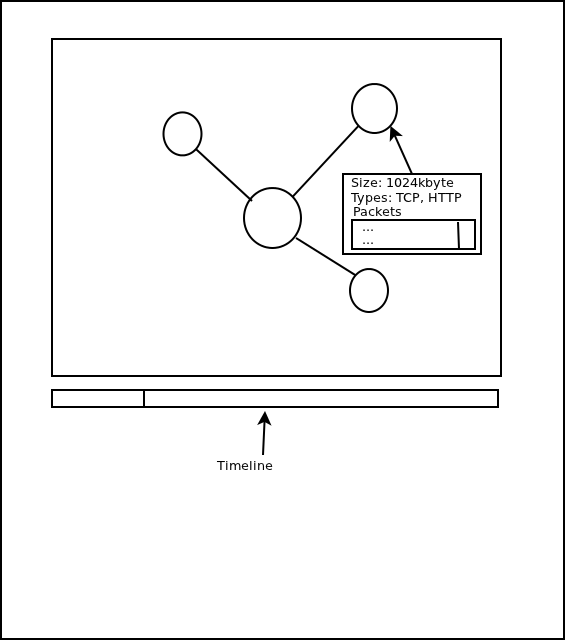
\includegraphics[width=0.9\textwidth]{./img/draft1.png}
 % draft1.png: 565x640 pixel, 72dpi, 19.93x22.58 cm, bb=0 0 565 640
 \caption{First design of the system.}
 \label{fig:draft1}
\end{figure}
\end{frame}



\subsection{Problems The 1st}

\begin{frame}
 \begin{enumerate}
  \item Web != Client application
  \item Javascript...
  \begin{enumerate}
   \item Single threaded
   \item When something ``is being done'', user cannot interact
   \item Packet transfer (AJAX) pauses everything...
  \end{enumerate}
  \item So we couldnt simulate something AND be responsive

 \end{enumerate}

\end{frame}

\subsection{Second Design}

\begin{frame}{(Reduced) Ideas}
 \begin{enumerate}
  \item Let the user set a point in timeline and show the state at that time
  \item No ``fancy'' simulation stuff
  \item The rest should remain the same
 \end{enumerate}

\end{frame}


\begin{frame}{And more problems...}
 \begin{enumerate}
  \item Packets... so many packets
  \item Even a short tcpdump generates a few thousand packets
  \item Transfer every packet from server to client?
  \item Reduced information which is sent to client
 \end{enumerate}
\end{frame}

\section{Demo}

\begin{frame}{The result}
\begin{enumerate}
 \item \url{http://tcpdumpnetworkvisualizer.appspot.com}
 \item Or just a video...
\end{enumerate}
\end{frame}

\begin{frame}{Optimal solution...}
\begin{enumerate}
 \item Use GWT for client-side javascript generation (Java is much better to maintain than JS)
 \item Write (or wait for) a GWT-InfoVis wrapper (offers features which are hard to implement)
\end{enumerate}
\end{frame}


\begin{frame}
  Thanks for your attention!
\end{frame}


\section{Referenzen}

\begin{frame}{References}
\printbibliography
\end{frame}


\end{document}
